\subsection{Tempo de vida a partir das oscilações radiais}
Na análise anterior considerou-se que a probabilidade de um elétron passar por uma coordenada $s$ com deslocamento radial entre $x$ e $x+dx$ é distribuída conforme uma Gaussiana -- dada por
\begin{align}
	w(x)dx = \frac{1}{\sqrt{2\pi} \sigma_x}\ e^{-x^2/2\sigma_x^2}dx\label{eq:5.116}
\end{align}
com $\sigma_x$ uma função de $s$. É claro que esta distribuição não é completamente correta uma vez que esta possui "caudas" que se estendem até grandes valores de deslocamento, tanto positivos quanto negativos, enquanto que, em um anel de armazenamento real, o feixe deve se manter dentro da câmara de vácuo, a qual tem abertura finita. Logo, a função de probabilidade da equação \eqref{eq:5.116} pode ser apenas uma aproximação, a qual é bem razoável com tanto que a abertura da câmara de vácuo seja bem maior que $\sigma_x$ em todo o anel.

No entanto, mesmo quando a abertura é grande, podem haver efeitos significantes desta limitação. Cedo ou tarde o elétron irá ter uma flutuação suficientemente grande durante sua emissão quântica a qual produzirá uma deslocamento do tamanho do limite da abertura dinâmica. Então, este elétron será perdido devido à colisão com a câmara de vácuo -- ou qualquer outra coisa que defina o limite da abertura dinâmica. De forma alternativa, considerando as não-linearidades do campo guia, amplitudes de oscilação maiores podem se tornar instáveis, causando a perda do elétron do feixe. Será conveniente nesta discussão pensar em termos de uma abertura dinâmica limitada por um obstáculo físico. Uma extensão deste raciocínio a uma abertura limitada por forças magnéticas é direta.

Com tanto que a chance de um elétron se perder no limite da abertura seja pequena -- ou seja, que esta seja muito menor que 1 em um tempo de amortecimento -- a probabilidade por unidade de tempo de se perder é a mesma para todos os elétrons. Então a taxa de perda será proporcional ao número $N$ de elétrons presentes; e $N$ irá, portanto, decrescer exponencialmente com uma constante de tempo $\tau_q$ ligada à taxa de perda por
\begin{align}
	\frac{1}{\tau_q} = -\frac{1}{N} \frac{dN}{dt}
\end{align}
O número $\tau_q$ é chamado de tempo de vida quântico do feixe de elétrons.

Uma análise precisa do tempo de vida quântico para todas as condições é um pouco complicada. Logo, uma forma de computá-lo será mostrada, a qual é razoavelmente precisa enquanto o tempo de vida seja grande -- que é a condição de maior interesse em um anel de armazenamento. Primeiramente, o tempo de vida devido às oscilações laterais será analisado. Em seguida, será analisado o tempo de vida devido às oscilações de energia.

Pense agora numa situação simplificada em que apenas as oscilações betatron radiais são excitadas -- ignorando por agora o \textit{spread} radial associado às oscilações de energia.  Na \autoref{sec:2.6} foi visto que, na ausência de efeitos quânticos, as oscilações betatron de um elétron se mantém entre o envelope $X(s) = a\sqrt{\beta(s)}$ -- veja a \autoref{fig:fig12}. Quando os efeitos quânticos e o amortecimento por radiação são considerados, a amplitude "invariante" $a$ de qualquer elétron varia de forma aleatória. A escala temporal da variação de $a$ é, no entanto, lenta -- isto é, muito maior que o período de revolução -- então pode-se pensar que o elétron continuamente varre uma banda radial cujo envelope varia lentamente.

Suponha que em alguma azimutal qualquer $s_1$ uma obstrução defina o limite da abertura dinâmica do anel. Isto é, quando a amplitude invariante $a$ varia, o envelope $X(s)$ irá encontrar um obstáculo em $s_1$. Veja a \autoref{fig:fig46}. Todas as perdas irão ocorrer em $s_1$, e apenas a distribuição radial precisa ser considerada nesta coordenada.

\begin{figure}[!htb]
	\centering
	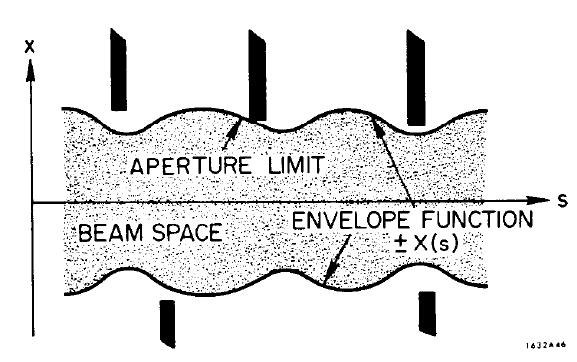
\includegraphics[width=0.6\linewidth]{./Figuras/fig46.jpeg}
	\caption{Limite da abertura dinâmica radial. Retirado de \cite{sands1970physics}.}
	\label{fig:fig46}
\end{figure}

Foi visto na \autoref{sec:2.7} que o deslocamento radial em sucessivas passagens coordenada em particular varia com o tempo conforme
\begin{align}
	x = a\sqrt{\beta_1}\ cos(\omega t)
\end{align}
Como foi feito na \autoref{sec:5.3} para as oscilações de energia, pode-se tomar o quadrado da amplitude como uma medida da "energia efetiva" das oscilações. Então, define-se
\begin{align}
	W = a^2 \beta_1
\end{align}
Efeitos quânticos e amortecimento por radiação produzem flutuações de variação lente em $W$. Os mesmos argumentos utilizados na \autoref{sec:5.3} podem ser usados aqui para mostrar que -- na ausência de qualquer limite de abertura -- os elétrons de um feixe terão uma distribuição de $W$ de acordo com (veja a equação \eqref{eq:5.62})
\begin{align}
	h(W) = \frac{N}{\mean{W}}\ e^{-W/\mean{W}}\label{eq:5.120}
\end{align}
onde o valor médio $\mean{W}$ é igual a $2\sigma_x^2$ (a função $h(W)$ é definida de forma que o número de elétrons com "oscilação de energia" entre $W$ e $W+dW$ é $h(W)dW$). A função $h(W)$ é mostrada na \autoref{fig:fig47}

\begin{figure}[!htb]
	\centering
	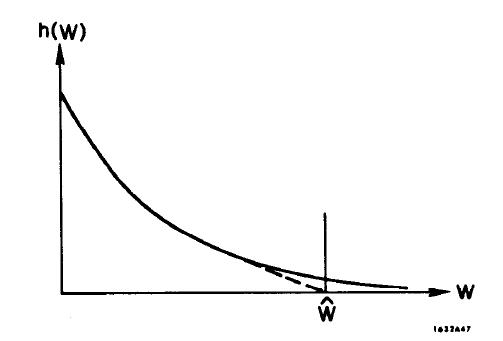
\includegraphics[width=0.6\linewidth]{./Figuras/fig47.jpeg}
	\caption{Distribuição das oscilações de energia. Retirado de \cite{sands1970physics}.}
	\label{fig:fig47}
\end{figure}

Agora considere o que acontece quando existe um limite de abertura que remove qualquer elétron cujo $W$ excedo um limiar $\hat{W}$ -- o qual é chamado de "$W$ de pico". Não existem elétrons com $W > \hat{W}$, então a distribuição atual $h(W)$ deve mudar para grandes valores de $W$ de forma semelhante à curva tracejada da \autoref{fig:fig47}. Pode-se pensar no que está acontecendo da seguinte maneira. Os efeitos quânticos estão continuamente tentando preencher a distribuição ideal com uma "difusão" dos elétrons da região de baixo $W$ para a região de grande $W$. Mas cada vez que um elétron alcança $\hat{W}$ ele é "varrido para fora", então há uma perda contínua na perda por radiação da distribuição. Pode-se estimar esta taxa de perda.

Pode-se fazer uma estimativa grosseira da seguinte maneira. Foi dito que o "tempo de relaxamento" característico das flutuações quânticas é igual à constante de tempo de amortecimento $\tau_x$. Desta forma, pode-se chutar que há uma "tentativa" de preencher a perda por radiaçãoão da distribuição ideal a cada tempo de amortecimento. Então o número de elétrons perdidos em cada tempo de amortecimento será igual ao número de elétrons na distribuição ideal com $W> \hat{W}$. Este número é
\begin{align}
	N(>\hat{W}) = \int\limits_{\hat{W}}^{\infty}h(W)dW = N\ e^{-\hat{W}/\mean{W}}
\end{align}
A taxa de perda dos elétrons será estimada por
\begin{align}
	-\frac{dN}{dt} \approx \frac{N}{\tau_x}\ e^{-\hat{W}/\mean{W}}
\end{align}
que resultará em um tempo de vida quântico de
\begin{align}
	\tau_q \approx \tau_x\ e^{\hat{W}/\mean{W}}\label{eq:5.123}
\end{align}
Ou seja, o tempo de vida depende exponencialmente de $\hat{W}/\mean{W}$.

Um cálculo mais exato de $\tau_q$ requer que uma equação de difusão para $h(W)$ seja definida e que esta seja resolvida numericamente com condições de contorno apropriadas. Este tipo de análise não será feita aqui, no lugar será mostrado como uma boa aproximação pode ser obtida.

Considere o que aconteceria na vizinhança de algum $W_0$ muito maior que $\mean{W}$ caso não existisse um limite de abertura. A chance de achar qualquer elétron com $W>W_0$ na distribuição ideal é muito pequena. Espera-se, então, que uma vez que um elétron entre na perda por radiação ($W>W_0$) é mais provável que ele retorne rapidamente ao corpo da distribuição -- seu lugar na perda por radiação sendo reposto por outro elétron sem sorte. Considere agora o fluxo de elétrons passando por uma pequena zona\footnote{Pensando na passagem por uma "zona", pode-se ignorar as flutuações microscópicas da amplitude.} próxima de $W_0$. Os elétrons posicionados na perda por radiaçãoão irão passar para o lado esquerdo por esta zona e um fluxo igual de elétrons irão (em condições estacionárias) passar para o lado direito pela mesma zona devido a flutuações quânticas anormais. Neste pensamento, eventos improváveis onde o elétron deixando a cauda teria flutuações anormais neste instante e entraria novamente na cauda não são considerados.

Hora de estimar o fluxo de elétrons saindo da cauda. Quando $W$ é grande, as flutuações "normais" de energia podem ser negligenciadas em comparação com a taxa de de decrescimento de $W$ devido ao amortecimento. Para qualquer elétron, o amortecimento resulta em
\begin{align}
	\frac{dW}{dt} = -\frac{2W}{\tau_x}
\end{align}
e o fluxo de elétrons passando por $W_0$ devido ao amortecimento será
\begin{align}
	\left\{h(W) \frac{dW}{dt}\right\}_{W_0} = \frac{2W_0 h(W_0)}{\tau_x}\label{eq:5.125}
\end{align}

Na ausência de um limite de abertura, o fluxo líquido por qualquer $W$ -- em particular, por $W_0$ -- deve ser zero para que exista um fluxo de elétrons para dentro da cauda igual ao fluxo para fora descrito pela equação \eqref{eq:5.125}.

Agora, considere um limite de abertura em $\hat{W}$. Se este limite é suficientemente grande, o corpo da distribuição é pouco afetado. O fluxo saindo do corpo por $\hat{W}$ não será alterado enquanto, obviamente, o fluxo para dentro da distribuição será zero. Tem-se que o fluxo da equação \eqref{eq:5.125} avaliado em $W_0= \hat{W}$ também é uma estimativa do fluxo para fora de elétrons perdidos. Então, a taxa de perda será
\begin{align}
	-\frac{dN}{dt} = \frac{2\hat{W} h(\hat{W})}{\tau_x}
\end{align}
Utilizando a equação \eqref{eq:5.120} para $h(W)$, obtém-se que
\begin{align}
	\tau_q = \frac{\tau_x}{2} \frac{\mean{W}}{W}\ e^{\hat{W}/\mean{W}}\label{eq:5.127}
\end{align}
Lembre-se que $\hat{W}$ e $\mean{W}$ são relacionados com a excursão máximo radial permitida pela abertura (o qual ocorre em alguma azimutal $s_1$) e o deslocamento radial RMS nesta coordenada por
\begin{align}
	\hat{W} = [a^2 \beta_x(s_1)]_{max}\ \ \ \ \ \ \ \mean{W} = 2\sigma_x^2(s_1)
\end{align}
com ambos avaliados na posição azimutal do limite da abertura.

Este resultado difere do que foi estimado na equação \eqref{eq:5.123} por um fator $\mean{W}/2\hat{W}$, resultando, portanto, em um tempo de vida menor por um fator de 5 ou 10, geralmente. Esta discrepância pode ser explicada pelo argumento de que o "tempo de relaxamento" é menor por este fator para a população da cauda da distribuição do que para a população do corpo da mesma -- o que é plausível dado que uma flutuação maior tem mais chance de dominar o amortecimento por radiação se esta se acumular em um período de tempo relativamente curto. Apesar da equação \eqref{eq:5.127} ter sido derivada através de algumas aproximações cujos significados quantitativos não forame estimados, o mesmo resultado foi obtido com um cálculo mais sofisticado -- mas ainda aproximado.

Nesta derivação do tempo de vida quântico, assumiu-se que as flutuações radiais eram causadas apenas pelas oscilações betatron. No entanto, como foi visto na \autoref{sec:5.5} que o \textit{spread} radial do feixe tem contribuições tanto das oscilações betatron quanto das oscilações de energia. E a análise é complicada pelo fato de que cada componente tem uma constante de tempo diferente. Ao invés de tentar refinar o cálculo realizado, alguns comentários serão feitos. Primeiro, as duas constantes de tempo não são tão diferentes -- geralmente diferem por um fator 2. Então fica claro que a equação \eqref{eq:5.125} resulta em uma aproximação razoável se para $\sigma_x^2$ for usado o quadrado médio do \textit{spread} total do feixe e para $\tau_x$ algum valor entre as constantes de tempo betatron e do amortecimento síncrono. Ou, de forma alternativa, pode-se obter uma estimativa "segura" de $\tau_q$ -- isto é, seu valor mínimo -- usando para $\tau_x$ a menor entre as duas constantes de tempo.

O tempo de vida quântico aumenta aproximadamente de forma exponencial com o quadrado da excursão máxima radial --  uma variação extremamente rápida. Sendo assim, um critério mais preciso para a abertura dinâmica é necessário. Se a abertura é um pouco menor, o tempo de vida será desastrosamente menor; da mesma forma, se a abertura é um pouco maior, o tempo de vida será astronomicamente maior e não terá nenhuma consequência\footnote{Já que outros mecanismos de perda irão, então, dominar o processo.}. O limite de abertura "crítico" ocorre em torno de
\begin{align}
	\frac{|x_{max}|}{\beta_x} = 6\sigma_x
\end{align}
o que resulta em $\hat{W}/\mean{W} \approx 18$ e, pela equação \eqref{eq:5.127},
\begin{align}
	\tau_q = \frac{\tau_x}{36}\ e^{18} \approx 1.5 \times 10^6 \tau_x
\end{align}
Como $\tau_x$ é tipicamente em torno de 0.1 segundos. A abertura crítica resulta em uma tempo de vida quântico de mais ou menos 1 dia. Outros efeitos como espalhamento de gases resultam em tempos de vida de algumas horas e o período de injeção (tempo necessário para armazenar o feixe de elétrons) é geralmente de um fração de hora, então o tempo de vida de um dia é um tanto quanto "seguro". Assim, pode-se entender à "regra do polegar\footnote{Expressão que caracteriza um método comumente aceito o qual se baseia no conhecimento prático, não tendo embasamento científico.}" de que a abertura total deve ser ao menos 12 vezes o desvio padrão $\sigma_x$ da distribuição radial. Uma regra similar se aplica à abertura vertical.